\documentclass{article}
\usepackage[utf8]{inputenc}
\usepackage[margin=1in]{geometry}

\title{452 - Homework 3}
\author{Victor Zhang}
\date{February 12, 2021}

\usepackage[utf8]{inputenc}
\usepackage{amsmath}
\usepackage{amsfonts}
\usepackage{natbib}
\usepackage{graphicx}
% \usepackage{changepage}
\usepackage{amssymb}
\usepackage{xfrac}
% \usepackage{bm}
% \usepackage{empheq}
\usepackage{tikz}
\usetikzlibrary{arrows,automata}

\newcommand{\contra}{\raisebox{\depth}{\#}}

\newenvironment{myindentpar}[1]
  {\begin{list}{}
          {\setlength{\leftmargin}{#1}}
          \item[]
  }
  {\end{list}}

\pagestyle{empty}

\begin{document}

\maketitle
% \begin{center}
% {\huge Econ 482 \hspace{0.5cm} HW 3}\
% {\Large \textbf{Victor Zhang}}\
% {\Large February 18, 2020}
% \end{center}

\section*{1.21.a}
Removing state 1, we may write the transition from start to state 2 as $a^*b$ and subsequent transitions as $(ba^*b)\cup a$. Then the regular expression corresponding to the machine is $a^*b((ba^*b)\cup a)^*$ $\Box$

\section*{1.21.b}
Let us first construct a GNFA from the given machine.

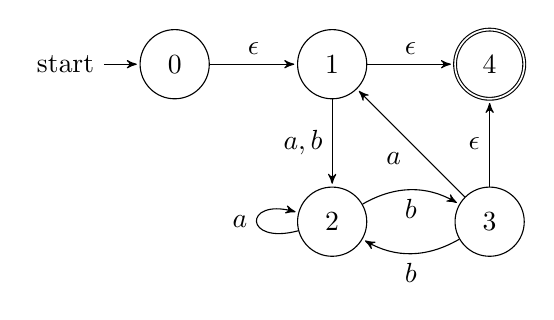
\begin{tikzpicture}[->,>=stealth',shorten >=1pt,auto,node distance=2cm,
        scale = 1,transform shape]

  \node[state,initial] (0) {$0$};
  \node[state] (1) [right of=0] {$1$};
  \node[state] (2) [below of=1] {$2$};
  \node[state] (3) [right of=2] {$3$};
  \node[state,accepting] (4) [right of=1] {$4$};

  \path (0) edge              node {$\epsilon$} (1)
        (1) edge              node [left] {$a,b$} (2)
        (1) edge              node {$\epsilon$} (4)
        (2) edge [loop left]  node {$a$} (2)
        (2) edge [bend left]  node [below] {$b$} (3)
        (3) edge [bend left]  node {$b$} (2)
        (3) edge              node {$a$} (1)
        (3) edge              node {$\epsilon$} (4);

\end{tikzpicture}

\noindent
Now remove states

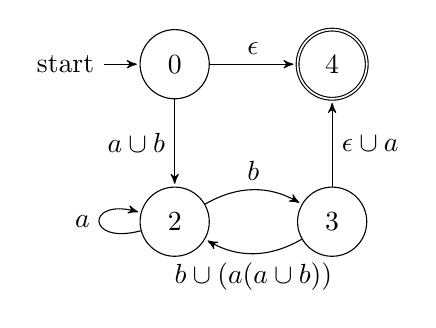
\begin{tikzpicture}[->,>=stealth',shorten >=1pt,auto,node distance=2cm,
        scale = 1,transform shape]

  \node[state,initial] (0) {$0$};
  \node[state] (2) [below of=0] {$2$};
  \node[state] (3) [right of=2] {$3$};
  \node[state,accepting] (4) [right of=0] {$4$};

  \path (0) edge              node [left] {$a \cup b$} (2)
        (0) edge              node {$\epsilon$} (4)
        (2) edge [loop left]  node {$a$} (2)
        (2) edge [bend left]  node {$b$} (3)
        (3) edge [bend left]  node {$b \cup (a(a \cup b))$} (2)
        (3) edge              node [right] {$\epsilon \cup a$} (4);

\end{tikzpicture}
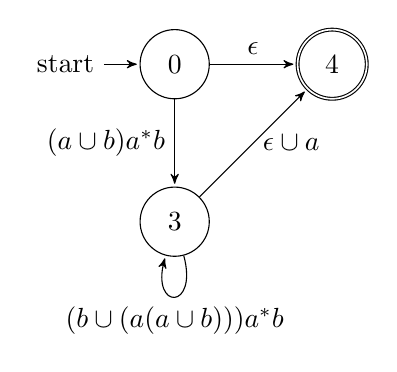
\begin{tikzpicture}[->,>=stealth',shorten >=1pt,auto,node distance=2cm,
        scale = 1,transform shape]

  \node[state,initial] (0) {$0$};
  \node[state] (3) [below of=0] {$3$};
  \node[state,accepting] (4) [right of=0] {$4$};

  \path (0) edge              node [left] {$(a \cup b)a^*b$} (3)
        (3) edge [loop below] node {$(b \cup (a(a \cup b)))a^*b$} (3)
        (3) edge              node [right] {$\epsilon \cup a$} (4)
        (0) edge              node {$\epsilon$} (4);

\end{tikzpicture}

\noindent
So the final reg. exp. is $((a \cup b)a^*b((b \cup (a(a \cup b)))a^*b)^*(\epsilon \cup a)) \cup \epsilon$ $\Box$

\section*{1.29.b}
Take arbitrary $p$ and let $w = 010010001\dots0^k1$ s.t. $|w| \geqslant p+1$. Then as specified by the pumping lemma, put $xyz = www$. Since $|xy| \leqslant p$, $xy^0z \notin A_2$. Then by the pumping lemma, $A_2$ is not regular $\Box$

\section*{1.32}
We construct an NFA for the reverse of the language. That is, instead of reading numbers with the high bit first, we read numbers with the high bit last. For simplicity of expression, we will represent a binary array as simply the digits concatenated. For example, $\left[\begin{smallmatrix}0\\1\\0\end{smallmatrix}\right]$ we will write as $010$.

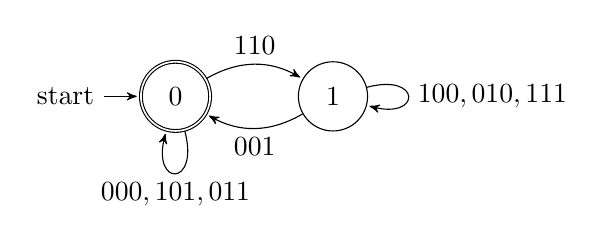
\begin{tikzpicture}[->,>=stealth',shorten >=1pt,auto,node distance=2cm,
        scale = 1,transform shape]

  \node[state,accepting,initial] (0) {$0$};
  \node[state] (1) [right of=0] {$1$};

  \path (0) edge [loop below] node {$000,101,011$} (0)
        (0) edge [bend left]  node {$110$} (1)
        (1) edge [loop right] node {$100,010,111$} (1)
        (1) edge [bend left]  node {$001$} (0);

\end{tikzpicture}

\noindent
If desired, we may construct a DFA from this NFA by simply pointing all other possible transitions to an absorbing non-accepting state $q$. Since we may construct a NFA (and DFA) that accepts $B^{\mathcal{R}}$, $B^\mathcal{R}$ and thus $B$ is regular $\Box$

\section*{1.35}
Pick arbitrary $p$ and let $s = \left[\begin{smallmatrix}0\\1\end{smallmatrix}\right]^p \left[\begin{smallmatrix}0\\0\end{smallmatrix}\right] \left[\begin{smallmatrix}1\\0\end{smallmatrix}\right]^p$. Clearly, $s \in E$ and $|s| = 2p+1$. Then let $s = xyz$ as in the pumping lemma. Note $y = \left[\begin{smallmatrix}0\\1\end{smallmatrix}\right]^j$ for some $j \leq p$. Then clearly $xy^0z \notin E$. By the pumping lemma, $E$ is not regular $\Box$

\section*{1.40.b}
Suppose $A$ is regular and $M = (Q,\Sigma,\delta,q_0,F)$ is a DFA that accepts $A$. Build NFA $M' = (Q \cup \{q_F\}, \Sigma, \delta', q_0, \{q_F\})$ where the transition function is modified from $\delta$ to not include any transitions out of $F$, except a null transition to $q_F$. That is, the machine operates exactly as $M$, except reaching a state $g \in F$ immediately transitions to the final (accepting) state. We claim this accepts $NOEXTEND(A)$.\\
Indeed, $M'$ never accepts strings $w \notin NOEXTEND(A)$. If $w \notin A$ this is clear, since $M'$ does not add any substantive transitions or states. If $w \in A$ has a prefix $w'$ which is also accepted, it must enter some state $g \in F$, whereupon $M'$ would send it to $q_F$ and then die after receiving more input. So it follows that no $w \in L(M')$ has a prefix. Also note every $v \in A$ which is not a prefix is accepted. Since transitions between non-accepting states and into accepting states are preserved, $v$ is accepted as well. Hence, $M'$ accepts exactly $NOEXTEND(A)$ $\Box$

\section*{1.46.a}
Pick arbitrary $p$ and let $s = 0^p10^p$. Clearly, $s$ is in the language. Write $s = xyz$ as in the pumping lemma. Suppose $|y| = j$. Since $|xy| \leq p$, it follow that $xy^0z = 0^{p-j}10^p$, which is not in the language. By the pumping lemma, this language is not regular $\Box$

\section*{1.46.c}
The string $s$ from the previous section is a palindrome. Thus, we may repeat the proof to show the set $A$ of palindromes is not regular. Then $A^C$, the language we are interested in, must not be regular either $\Box$

\section*{1.46.d}
Pick arbitrary $p$ and let $s$ be as in section 1.46.a. $s$ is in the language, and we may repeat the pumping lemma proof to show the language is not regular $\Box$

\section*{1.49.a}
Consider a string $s = 1^ky \in B$. If $k > 1$, we may write $s = 1y'$, where $y' = 1^{k-1}y$. Thus, we may represent $B = \{1y \;:\; y \text{ contains at least one 1}\}$. This language is accepted by the following NFA with $3$ states:

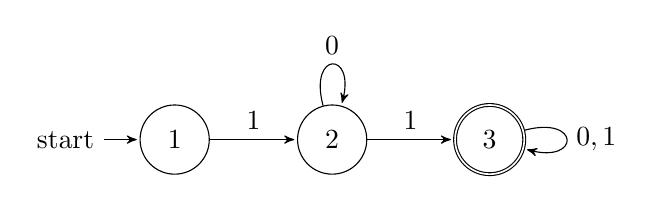
\begin{tikzpicture}[->,>=stealth',shorten >=1pt,auto,node distance=2cm,
        scale = 1,transform shape]

  \node[state,initial] (1) {$1$};
  \node[state] (2) [right of=1] {$2$};
  \node[state,accepting] (3) [right of=2] {$3$};

  \path (1) edge              node {$1$} (2)
        (2) edge              node {$1$} (3)
        (2) edge [loop above] node {$0$} (2)
        (3) edge [loop right] node {$0,1$} (3);

\end{tikzpicture}

\noindent
So the language is regular $\Box$

\section*{1.49.b}
Pick arbitrary $p$ and put $s = 1^p01^p \in C$. Let $x = xyz$ as in the pumping lemma. Then $y = 1^{j}$ for some $j \leqslant p$. But $xy^0z = 1^{p-j}01^p \notin C$, since $k < p$. Thus, by pumping lemma $C$ is not regular $\Box$

\end{document}

% List of tex snippets:
%   - tex-header (this)
%   - R      --> \mathbb{R}
%   - Z      --> \mathbb{Z}
%   - B      --> \mathcal{B}
%   - E      --> \mathcal{E}
%   - M      --> \mathcal{M}
%   - m      --> \mathfrak{m}({#1})
%   - normlp --> \norm{{#1}}_{L^{{#2}}}
